% ==========================================================================
\section{Computer Maintenance}
% ==========================================================================

    % ==========================================================================
    \subsection{Internal Battery}
    % ==========================================================================

    While it is switched off, the computer keeps the date and time, thanks to
    its Real-Time Clock (RTC) internal circuitry.

    This circuitry is supported by a LIR2032 Li-Ion Rechargeable 3.6V Battery
    Button Cell.

    Ideally, to maintain the battery at full charge, the computer SHOULD be
    switched on for at least one hour every month.

    After a few years, due the way rechargeable batteries work, the battery may
    be unable to recharge anymore. In such case, the baterry MUST be replaced
    with a new battery of the same characteristics.

    If you are not planning to use the computer for a year or more, it is highly
    recommended to remove the battery, to avoid leacking of chemical liquids
    that are highly toxic but also can damage the internal circuitry.

    To replace/remove the battery you need to open the computer case. To do so,
    unscrew the three small cross-head screws under the front edge of the
    computer case.

    \centerline{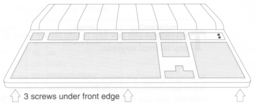
\includegraphics[scale=1]{images/keyboardscrews.png}}

    There is no danger of electrical shock, as the computer is power just by 5V,
    but it is highly recommended to unplug the computer to avoid possible short
    circuits that could damage the internal circuitry. It is also recommened to
    discharge yourself from static electricity before touching the inside of the
    computer.

    % ==========================================================================
    \subsection{Cleaning the computer}
    % ==========================================================================

    In general, avoid high humidity, extreme cold, and extreme heat environments.

    It is highly recommended to use a cover to avoid the concentration of dust
    in the keyboard, which can lead to false contacts.

    Do not put the computer in the dishwasher!